\section{Hidden Markov Models}
\subsection{Introduction to Hidden Markov Models (Chains)}
For Markov chains, the assumptions may be restrictive. The state of the variable may not be fully observed; instead, each state is contributed by a hidden variable $z_i$.
\begin{figure}[H]
    \centering
    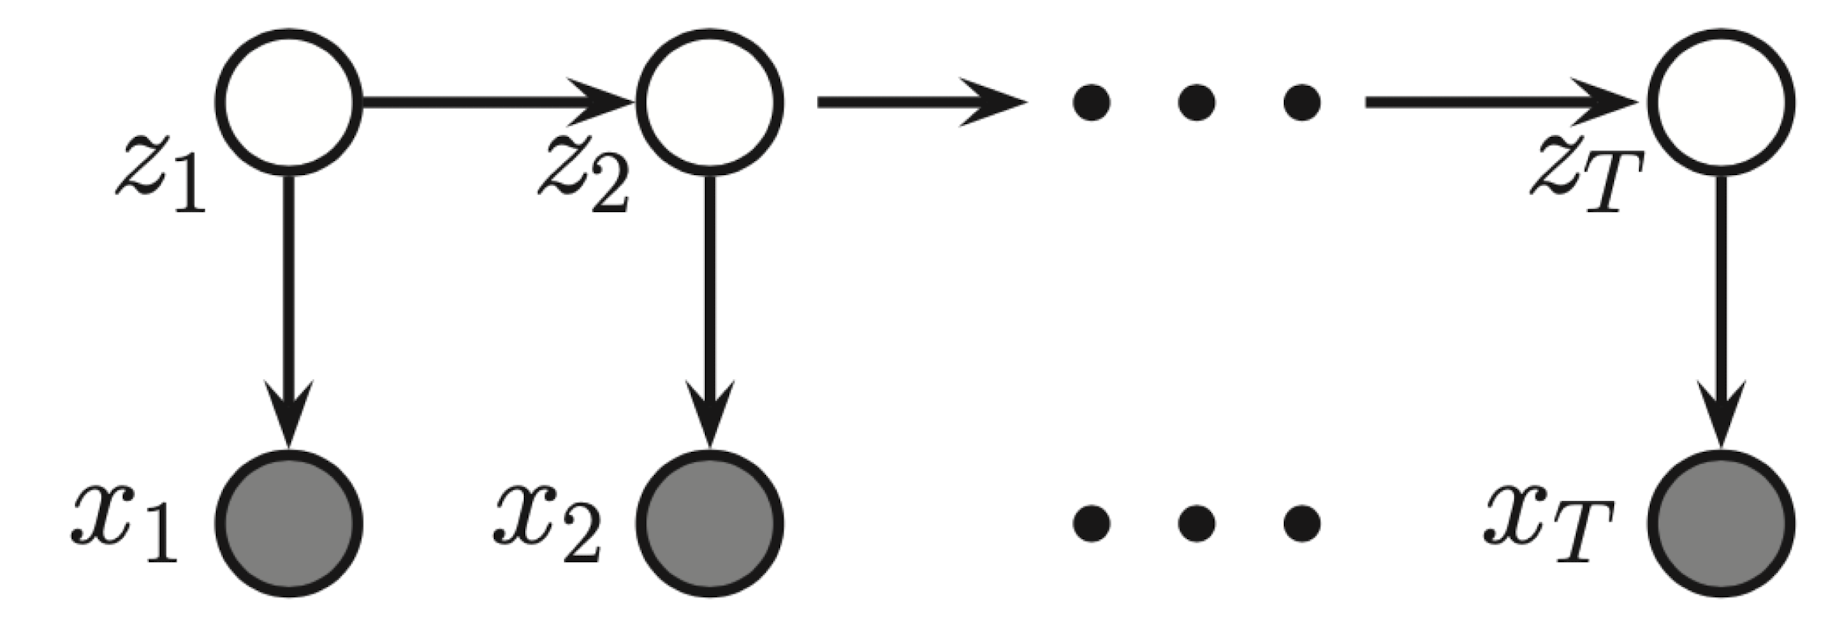
\includegraphics[width = .4\linewidth]{codes/figures/section7/figure_7_1.png}
    \caption{An example of Hidden Markov Chain}
    \label{fig:hidden_markov_chain}
\end{figure}
Above is an example of Hidden Markov Chain. It hides the temporal dependence by keeping it as unobserved state. For each observation $x_t$, we associated it with a \textbf{hidden/latent} state $z_t$. The joint distribution can be written as:
$$p\left(x_{1: T}, z_{1: T}\right)=p\left(z_1\right) \prod_{t=2}^T p\left(z_t \mid z_{t-1}\right) \prod_{t=1}^T p\left(x_t \mid z_t\right)$$
Hidden Markov Models are not limited by the assumptions of Markov Chains. In HMMs, we only need to know three sets of distributions:
\begin{enumerate}
    \item \textbf{Initial distribution}. This is the probability of the first hidden state being $i$
    $$\pi(i)=p(z_1=i)$$
    \item \textbf{Transition distribution}. The probability of hidden state of transition from state $i$ to $j$.
    $$A_{ij}=p(z_{t+1}=j|z_t=i)$$
    \item \textbf{Emission probability}. The probability of an observed random variable $x_t$ given its hidden variable.
    $$p(x_t=j|z_t=i)$$
\end{enumerate}
Moreover, we have two main objectives.
\begin{enumerate}
    \item We want to compute the probability of a laten sequence given an observed sequence, which is:
    $$p(z_{1:t}|x_{1:t})$$
    This is achieved by \textbf{Forward-backward algorithm}
    \item Find the most likely unobservable sequence.
    $$z^{\star}=\underset{z_{1: T}}{\operatorname{argmax}} p\left(z_{1: T} \mid x_{1: T}\right)$$
    using the \textbf{Viterbi algorithm}
\end{enumerate}

\subsection{Forward-backward algorithm}
This task of hidden state inference breaks down into the following:
\begin{itemize}
    \item \textbf{Filtering}: compute posterior over current hidden state, $p\left(z_t \mid x_{1: t}\right)$.
    \item \textbf{Prediction}: compute posterior over future hidden state, $p\left(z_{t+k} \mid x_{1: t}\right)$.
    \item \textbf{Smoothing}: compute posterior over past hidden state, $p\left(z_t \mid x_{1: T}\right) \quad 1 \leq t<T$.
\end{itemize}
\subsubsection*{Forward Recursion}
\textbf{Goal}: Compute the \textbf{filtered marginals}
$$\alpha_t(j)=p\left(z_t=j \mid x_{1: t}\right)$$
given the initial distribution, transition distribution and emission probability described above.
It has two steps:
\begin{enumerate}
    \item \textbf{Prediction step}: compute the one-step-ahead predictive density:
    $$
    \begin{aligned}
        p\left(z_t=j \mid x_{1:(t-1)}\right) & =\sum_{i=1}^K p\left(z_{t-1}=i, z_t=j \mid x_{1:(t-1)}\right) \\
        & =\sum_{i=1}^K p\left(z_t=j \mid z_{t-1}=i, x_{1:(t-1)}\right) p\left(z_{t-1}=i \mid x_{1:(t-1)}\right) \\
        & =\sum_{i=1}^K p\left(z_t=j \mid z_{t-1}=i\right) p\left(z_{t-1}=i \mid x_{1:(t-1)}\right)=\sum_{i=1}^K A_{i j} \alpha_{t-1}(i)=\left(A^{\top} \alpha_{t-1}\right)_j
    \end{aligned}
    $$
    \item \textbf{Update step}: Denoting $\lambda_t(j)=p\left(x_t \mid z_t=j\right)$ (here $x_t$ is fixed and $\lambda_t \in \mathbb{R}^K$ )
    $$
    \begin{aligned}
        \alpha_t(j) & =p\left(z_t=j \mid x_{1: t}\right)=p\left(z_t=j \mid x_{1:(t-1)}, x_t\right)\\
        & \propto p\left(z_t=j, x_t \mid x_{1:(t-1)}\right) \\
        & =p\left(x_t \mid z_t=j, x_{1:(t-1)}\right) p\left(z_t=j \mid x_{1:(t-1)}\right) \\
        & =p\left(x_t \mid z_t=j\right) p\left(z_t=j \mid x_{1:(t-1)}\right)=\lambda_t(j) p\left(z_t=j \mid x_{1:(t-1)}\right)
    \end{aligned}
    $$
\end{enumerate}
\subsubsection*{Backward Recursion}
\textbf{Goal}: Compute:
$$\beta_t(i) = p\left(x_{(t+1): T} \mid z_t=i\right)$$
\begin{align*} 
    \beta_t(i) & =p\left(x_{(t+1): T} \mid z_t=i\right)\\
    & =\sum_{j=1}^K p\left(z_{t+1}=j, x_{t+1}, x_{(t+2): T} \mid z_t=i\right) \\ 
    & =\sum_j p\left(x_{(t+2): T} \mid z_{t+1}=j, z_t=i, x_{t+1}\right) p\left(x_{t+1} \mid z_{t+1}=j, z_t=i\right) p\left(z_{t+1}=j \mid z_t=i\right) \\ 
    & =\sum_j p\left(x_{(t+2): T} \mid z_{t+1}=j\right) p\left(x_{t+1} \mid z_{t+1}=j\right) p\left(z_{t+1}=j \mid z_t=i\right) \\ 
    & =\sum_j \beta_{t+1}(j) \lambda_{t+1}(j) A_{i j}
\end{align*}
\subsubsection*{Smoothing}
In smoothing inference, We can break the chain into two parts, the past and the future, by conditioning on $z_t$ :
$$
\begin{aligned}
\gamma_t:=p\left(z_t \mid x_{1: T}\right) & \propto p\left(z_t, x_{1: T}\right)=p\left(z_t, x_{1: t}, x_{(t+1): T}\right) \\
& =p\left(z_t, x_{1: t}\right) p\left(x_{(t+1): T} \mid z_t, x_{1: t}\right)=p\left(z_t, x_{1: t}\right) p\left(x_{(t+1): T} \mid z_t\right) \\
& \propto p\left(z_t \mid x_{1: t}\right) p\left(x_{(t+1): T} \mid z_t\right) \\
& =(\text { Forward Recursion)(Backward Recursion) }
\end{aligned}
$$
- Here we use the conditional independence $x_{(t+1): T} \perp x_{1: t} \mid z_t$.\\
- We know how to perform forward recursion from the previous part.\\

After we complete the forward and backward recursion, we now can compute the marginal probabilities of $p(z_{1:t}|x_{1:t})$, $p(z_t|x_{1:T})$. 

\subsection{Viterbi Algorithm}
The Viterbi Algorithm is used to compute the most probable laten sequence.
$$\hat{z}=\arg \max _{z_{1: T}} p\left(z_{1: T} \mid x_{1: T}\right)$$
It is a specialized version of max-product inference. The forward pass uses max-product, and the backward use the traceback procedure to recover the most probable sequence. It works as follows:
\begin{enumerate}
    \item Define $\delta_t$ via
    $$
    \delta_t(j)=\max _{z_1, \ldots, z_{t-1}} p\left(z_{1:(t-1)}, z_t=j, x_{1: t}\right)
    $$
    which is the probability of ending up in state $j$ at time $t$, by taking the most probable path.
    \item Moreover,
    $$
    \begin{aligned}
        \delta_t(j) & =\max _{z_1, \ldots, z_{t-1}} p\left(z_{1:(t-1)}, z_t=j, x_{1:(t-1)}, x_t\right) \\
        & =\max _{z_1, \ldots, z_{t-1}} p\left(z_{1:(t-1)}, x_{1:(t-1)}\right) p\left(z_t=j \mid z_{t-1}\right) p\left(x_t \mid z_t=j\right) \\
        & =\max _i \max _{z_1, \ldots, z_{t-2}} p\left(z_{1:(t-2)}, z_{t-1}=i, x_{1:(t-1)}\right) p\left(z_t=j \mid z_{t-1}=i\right) p\left(x_t \mid z_t=j\right) \\
        & =\max _i \delta_{t-1}(i) A_{i j} \lambda_t(j)
    \end{aligned}
    $$
\end{enumerate}
Keep track of the most likely previous state: $\theta_t(j)=\arg \max _i \delta_{t-1}(i) A_{i j} \lambda_t(j)$.

In practice:
\begin{itemize}
    \item Initialize the algorithm with
    $$
    \delta_1(j)=p\left(z_1=j, x_1\right)=\pi_j \lambda_1(j) .
    $$
    \item and terminate with
    $$
    z_T^*=\arg \max _i \delta_T(i)
    $$
    \item Then, we compute the most probable sequence of states using traceback:
    $$
    z_t^*=\theta_{t+1}\left(z_{t+1}^*\right)
    $$
\end{itemize}